\begin{figure}[h]
    \centering
    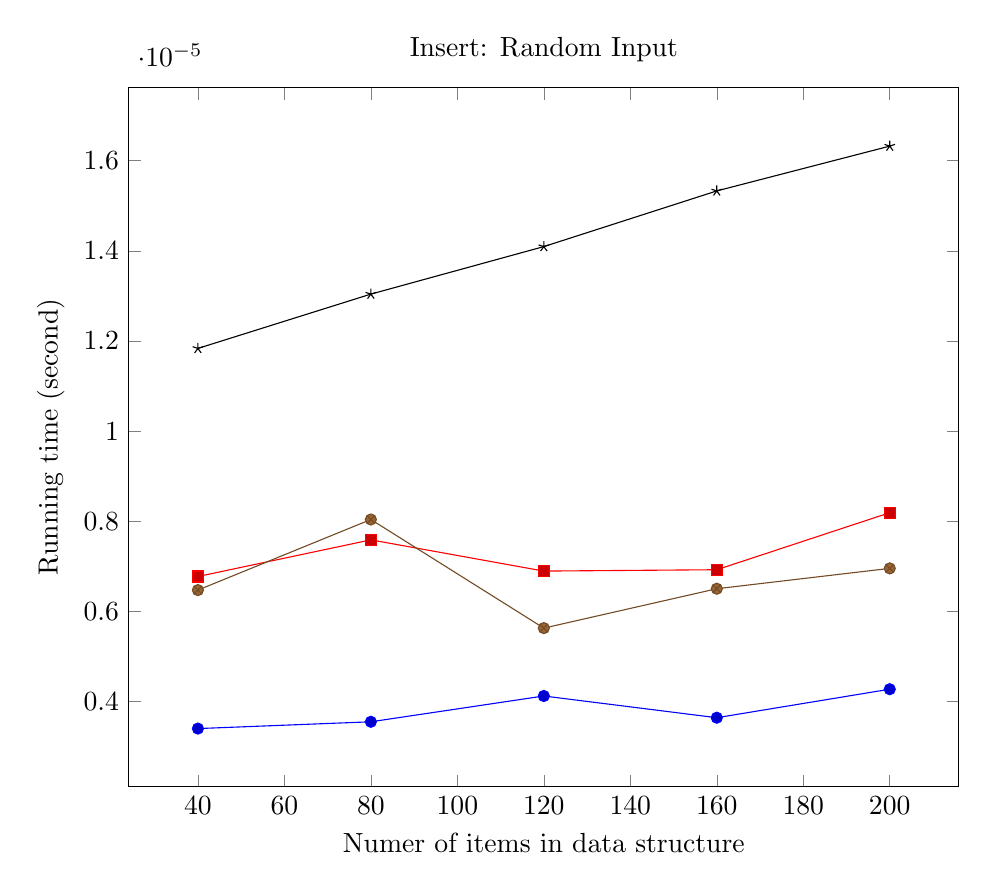
\begin{tikzpicture}
        \begin{axis}[
            xlabel={Numer of items in data structure},
            ylabel={Running time (second)},
            title={Insert: Random Input},
            width=\textwidth
        ]
		\addplot coordinates {
			(40, 3.403281305294076e-06)
			(80, 3.5538689736692996e-06)
			(120, 4.1261021134976485e-06)
			(160, 3.6442215746952666e-06)
			(200, 4.276689781873566e-06)
		};
		\addplot coordinates {
			(40, 6.776445076912829e-06)
			(80, 7.589618486142369e-06)
			(120, 6.896915211612731e-06)
			(160, 6.927032745288747e-06)
			(200, 8.191969159645345e-06)
		};
		\addplot coordinates {
			(40, 6.4752697401609934e-06)
			(80, 8.041381491269428e-06)
			(120, 5.631978797256132e-06)
			(160, 6.505387273836316e-06)
			(200, 6.957150278963376e-06)
		};
		\addplot coordinates {
			(40, 1.1836190734340612e-05)
			(80, 1.3040892081347261e-05)
			(120, 1.4095005759977991e-05)
			(160, 1.5329824640659962e-05)
			(200, 1.632370325194074e-05)
		};
        \legend{}
        \end{axis}
    \end{tikzpicture}
    \caption{Average of 0 operations, benchmarked every 0, starting at 0.}
\end{figure}